\definecolor{hfinitial}{HTML}{A37545}
\definecolor{hfind}{HTML}{78818E}
\definecolor{hfevo}{HTML}{00858B}
\definecolor{hfcontrol}{HTML}{B55D32}
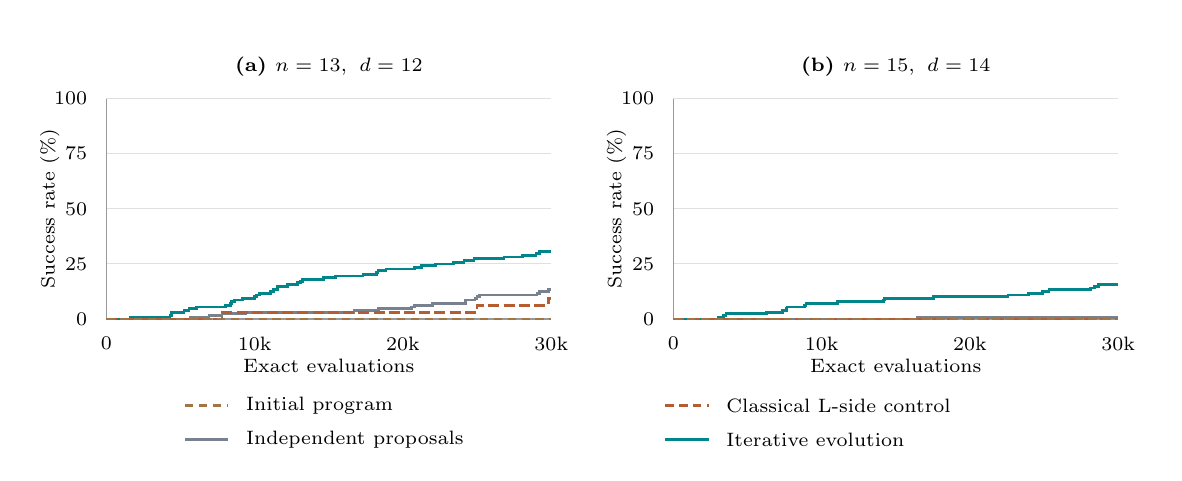
\begin{tikzpicture}[x=1cm,y=1cm,font=\scriptsize]
\path[use as bounding box] (-1,-1.70) rectangle (13.3,3.7);
\begin{scope}[xshift=0cm,yshift=0cm]
\node[font=\scriptsize\bfseries] at (2.825,3.2) {(a) $n=13,\ d=12$};
\draw[black!12,line width=.35pt] (0,0.0)--(5.65,0.0);
\node[anchor=east] at (-.12,0.0) {0};
\draw[black!12,line width=.35pt] (0,0.7)--(5.65,0.7);
\node[anchor=east] at (-.12,0.7) {25};
\draw[black!12,line width=.35pt] (0,1.4)--(5.65,1.4);
\node[anchor=east] at (-.12,1.4) {50};
\draw[black!12,line width=.35pt] (0,2.1)--(5.65,2.1);
\node[anchor=east] at (-.12,2.1) {75};
\draw[black!12,line width=.35pt] (0,2.8)--(5.65,2.8);
\node[anchor=east] at (-.12,2.8) {100};
\draw[black!40] (0,2.8)--(0,0)--(5.65,0);
\node[rotate=90] at (-.72,1.4) {Success rate (\%)};
\node at (2.825,-.60) {Exact evaluations};
\node[anchor=north] at (0.0,-.10) {0};
\node[anchor=north] at (1.8833333333333333,-.10) {10k};
\node[anchor=north] at (3.7666666666666666,-.10) {20k};
\node[anchor=north] at (5.65,-.10) {30k};
\draw[hfind,line width=1.0pt] (0.00000,0.00000) -- (1.07237,0.00000) -- (1.07237,0.02187) -- (1.30138,0.02187) -- (1.30138,0.04375) -- (1.46787,0.04375) -- (1.46787,0.06562) -- (1.76525,0.06562) -- (1.76525,0.08750) -- (3.14385,0.08750) -- (3.14385,0.10938) -- (3.45422,0.10938) -- (3.45422,0.13125) -- (3.87496,0.13125) -- (3.87496,0.15312) -- (3.91488,0.15312) -- (3.91488,0.17500) -- (4.14107,0.17500) -- (4.14107,0.19687) -- (4.55823,0.19687) -- (4.55823,0.21875) -- (4.55899,0.21875) -- (4.55899,0.24062) -- (4.68121,0.24062) -- (4.68121,0.26250) -- (4.70739,0.26250) -- (4.70739,0.28437) -- (4.73602,0.28437) -- (4.73602,0.30625) -- (5.46751,0.30625) -- (5.46751,0.32812) -- (5.50442,0.32812) -- (5.50442,0.35000) -- (5.61007,0.35000) -- (5.61007,0.37187) -- (5.65000,0.37187);
\draw[hfevo,line width=1.0pt] (0.00000,0.00000) -- (0.29964,0.00000) -- (0.29964,0.02187) -- (0.80776,0.02187) -- (0.80776,0.04375) -- (0.82377,0.04375) -- (0.82377,0.06562) -- (0.82528,0.06562) -- (0.82528,0.08750) -- (0.98404,0.08750) -- (0.98404,0.10938) -- (1.04808,0.10938) -- (1.04808,0.13125) -- (1.14883,0.13125) -- (1.14883,0.15312) -- (1.51194,0.15312) -- (1.51194,0.17500) -- (1.57334,0.17500) -- (1.57334,0.19687) -- (1.59236,0.19687) -- (1.59236,0.21875) -- (1.62362,0.21875) -- (1.62362,0.24062) -- (1.72702,0.24062) -- (1.72702,0.26250) -- (1.87900,0.26250) -- (1.87900,0.28437) -- (1.90763,0.28437) -- (1.90763,0.30625) -- (1.94153,0.30625) -- (1.94153,0.32812) -- (2.08598,0.32812) -- (2.08598,0.35000) -- (2.12120,0.35000) -- (2.12120,0.37187) -- (2.16979,0.37187) -- (2.16979,0.39375) -- (2.17299,0.39375) -- (2.17299,0.41562) -- (2.29691,0.41562) -- (2.29691,0.43750) -- (2.42310,0.43750) -- (2.42310,0.45937) -- (2.46867,0.45937) -- (2.46867,0.48125) -- (2.49353,0.48125) -- (2.49353,0.50312) -- (2.75833,0.50312) -- (2.75833,0.52500) -- (2.91069,0.52500) -- (2.91069,0.54688) -- (3.25986,0.54688) -- (3.25986,0.56875) -- (3.42955,0.56875) -- (3.42955,0.59062) -- (3.44951,0.59062) -- (3.44951,0.61250) -- (3.55121,0.61250) -- (3.55121,0.63437) -- (3.91074,0.63437) -- (3.91074,0.65625) -- (4.00623,0.65625) -- (4.00623,0.67812) -- (4.17780,0.67812) -- (4.17780,0.70000) -- (4.40399,0.70000) -- (4.40399,0.72187) -- (4.54147,0.72187) -- (4.54147,0.74375) -- (4.66728,0.74375) -- (4.66728,0.76562) -- (5.04790,0.76562) -- (5.04790,0.78750) -- (5.28840,0.78750) -- (5.28840,0.80937) -- (5.45507,0.80937) -- (5.45507,0.83125) -- (5.49594,0.83125) -- (5.49594,0.85312) -- (5.65000,0.85312);
\draw[hfcontrol,line width=1.0pt,dash pattern=on 4pt off 1.5pt] (0.00000,0.00000) -- (1.46787,0.00000) -- (1.46787,0.08750) -- (4.70739,0.08750) -- (4.70739,0.17500) -- (5.61007,0.17500) -- (5.61007,0.26250) -- (5.65000,0.26250);
\draw[hfinitial,line width=1.0pt,dash pattern=on 3pt off 2pt] (0.00000,0.00000) -- (5.65000,0.00000);
\end{scope}
\begin{scope}[xshift=7.2cm,yshift=0cm]
\node[font=\scriptsize\bfseries] at (2.825,3.2) {(b) $n=15,\ d=14$};
\draw[black!12,line width=.35pt] (0,0.0)--(5.65,0.0);
\node[anchor=east] at (-.12,0.0) {0};
\draw[black!12,line width=.35pt] (0,0.7)--(5.65,0.7);
\node[anchor=east] at (-.12,0.7) {25};
\draw[black!12,line width=.35pt] (0,1.4)--(5.65,1.4);
\node[anchor=east] at (-.12,1.4) {50};
\draw[black!12,line width=.35pt] (0,2.1)--(5.65,2.1);
\node[anchor=east] at (-.12,2.1) {75};
\draw[black!12,line width=.35pt] (0,2.8)--(5.65,2.8);
\node[anchor=east] at (-.12,2.8) {100};
\draw[black!40] (0,2.8)--(0,0)--(5.65,0);
\node[rotate=90] at (-.72,1.4) {Success rate (\%)};
\node at (2.825,-.60) {Exact evaluations};
\node[anchor=north] at (0.0,-.10) {0};
\node[anchor=north] at (1.8833333333333333,-.10) {10k};
\node[anchor=north] at (3.7666666666666666,-.10) {20k};
\node[anchor=north] at (5.65,-.10) {30k};
\draw[hfind,line width=1.0pt] (0.00000,0.00000) -- (3.09639,0.00000) -- (3.09639,0.02187) -- (5.65000,0.02187);
\draw[hfevo,line width=1.0pt] (0.00000,0.00000) -- (0.57065,0.00000) -- (0.57065,0.02187) -- (0.63337,0.02187) -- (0.63337,0.04375) -- (0.66953,0.04375) -- (0.66953,0.06562) -- (1.17897,0.06562) -- (1.17897,0.08750) -- (1.39103,0.08750) -- (1.39103,0.10938) -- (1.43359,0.10938) -- (1.43359,0.13125) -- (1.44471,0.13125) -- (1.44471,0.15312) -- (1.66204,0.15312) -- (1.66204,0.17500) -- (1.68408,0.17500) -- (1.68408,0.19687) -- (2.08447,0.19687) -- (2.08447,0.21875) -- (2.66850,0.21875) -- (2.66850,0.24062) -- (2.67716,0.24062) -- (2.67716,0.26250) -- (3.29903,0.26250) -- (3.29903,0.28437) -- (4.24880,0.28437) -- (4.24880,0.30625) -- (4.50550,0.30625) -- (4.50550,0.32812) -- (4.68366,0.32812) -- (4.68366,0.35000) -- (4.77067,0.35000) -- (4.77067,0.37187) -- (5.29876,0.37187) -- (5.29876,0.39375) -- (5.34471,0.39375) -- (5.34471,0.41562) -- (5.40328,0.41562) -- (5.40328,0.43750) -- (5.65000,0.43750);
\draw[hfcontrol,line width=1.0pt,dash pattern=on 4pt off 1.5pt] (0.00000,0.00000) -- (5.65000,0.00000);
\draw[hfinitial,line width=1.0pt,dash pattern=on 3pt off 2pt] (0.00000,0.00000) -- (5.65000,0.00000);
\end{scope}
\draw[hfinitial,line width=1pt,dash pattern=on 3pt off 2pt] (1,-1.1)--(1.55,-1.1);
\node[anchor=west] at (1.65,-1.1) {Initial program};
\draw[hfcontrol,line width=1pt,dash pattern=on 3pt off 2pt] (7.1,-1.1)--(7.6499999999999995,-1.1);
\node[anchor=west] at (7.75,-1.1) {Classical L-side control};
\draw[hfind,line width=1pt] (1,-1.53)--(1.55,-1.53);
\node[anchor=west] at (1.65,-1.53) {Independent proposals};
\draw[hfevo,line width=1pt] (7.1,-1.53)--(7.6499999999999995,-1.53);
\node[anchor=west] at (7.75,-1.53) {Iterative evolution};
\end{tikzpicture}
